\documentclass[tikz,border=8pt]{standalone}
\usepackage[utf8]{inputenc}
\usepackage[OT4,plmath]{polski}
\begin{document}
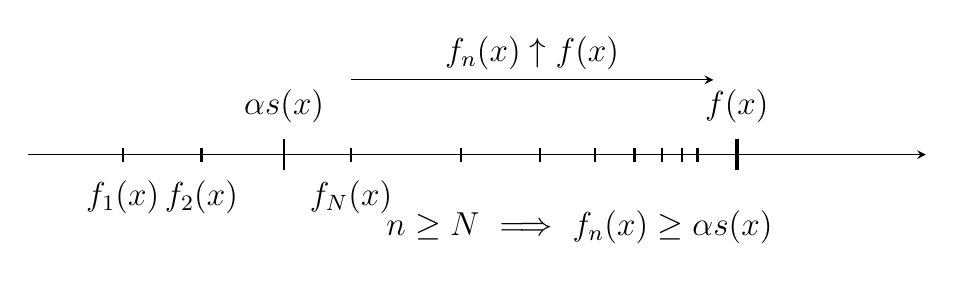
\begin{tikzpicture}[x=1cm,y=1cm,>=stealth,font=\large]
  \draw[->] (0,0) -- (11.4,0);
  \foreach \pos in {1.2,2.2,4.1,5.5,6.5,7.2,7.7,8.05,8.3,8.5} {
    \draw[thick] (\pos,-0.09) -- (\pos,0.09);
  }
  \node[below=6pt] at (1.2,0) {$f_1(x)$};
  \node[below=6pt] at (2.2,0) {$f_2(x)$};
  \draw[thick] (3.25,-0.2) -- (3.25,0.2);
  \node[above=8pt] at (3.25,0) {$\alpha s(x)$};
  \node[below=6pt] at (4.1,0) {$f_N(x)$};
  \draw[very thick] (9,-0.2) -- (9,0.2);
  \node[above=8pt] at (9,0) {$f(x)$};
  \draw[->] (4.1,0.95) -- (8.7,0.95);
  \node[above] at (6.4,0.95) {$f_n(x)\uparrow f(x)$};
  \node[below] at (7.0,-0.58) {$n\geq N\ \Longrightarrow\ f_n(x)\geq\alpha s(x)$};
\end{tikzpicture}
\end{document}
